% ====================================================================================
\chapter{机器人运动学与动力学}
% ====================================================================================

\section*{让机器动起来}

\storynote{Marc Raibert}{Boston Dynamics 创始人（1949--）。1980 年代他在 MIT 造出第一台单腿跳跃机器人，靠三条简单的控制律就让它站稳；后来的 BigDog、Atlas 都是这条路的延续。他的口头禅：“先让它跳起来，再想怎么落地。”}

\vspace{0.5cm}
\noindent\textit{你的手臂有7个自由度，但你从来不需要“计算”如何拿起一杯咖啡。机器人却需要——它必须把“拿杯子”这个任务翻译成每个关节应该转多少度。}

试着做一个实验：伸出你的手，保持手掌位置不动，然后移动你的手肘。你会发现，即使手掌固定，手肘仍然可以在一个圆弧上运动。这说明什么？你的手臂有“多余”的自由度——完成“固定手掌”这个任务后，还剩下一些自由度可以用来做别的事情。

这个简单的观察背后，是机器人学中一个核心问题：\textbf{运动学}——关节角度和末端位置之间的关系。更深一层，当机器人需要推、拉、抓取物体时，我们还需要\textbf{动力学}——力、质量、加速度之间的关系。

本章将展示：第5章学到的拉格朗日力学如何直接应用于机器人。你会发现，末端约束力、接触力都是拉格朗日乘子的工程化身，而关节力矩通过 $\tau = J^\top F$ 与它们相连。

\begin{quote}
\textbf{本章目标}：机器人是拉格朗日力学最直接的工程应用——把末端“钉”在目标上的约束力、脚与地面之间的接触力，都是第1章的拉格朗日乘子，只是这一次它们是真真切切的牛顿。本章将建立从“任务描述”到“关节力矩”的完整链条。
\end{quote}

\begin{tcolorbox}[colback=green!5, colframe=green!60!black, title=学完这章，你将能够...]
\begin{itemize}
    \item 用齐次变换建立机械臂的正运动学模型（D-H 参数是它的标准化写法）
    \item 计算雅可比矩阵，分析奇异构型
    \item 求解简单机械臂的逆运动学（解析解或数值解）
    \item 用拉格朗日方法推导机器人动力学方程
    \item 理解关节力矩与末端力的映射关系
\end{itemize}
\end{tcolorbox}

% ------------------------------------------------------------------------------------
\section{从人手臂到机械臂}

\subsection{为什么机器人需要“算”？}

人类拿起一杯咖啡，大脑只需要想“拿杯子”，手臂就自动完成了。我们从不需要计算“肩关节转23度，肘关节转45度，腕关节转-12度”。这件事在人看来毫不费力，对机器却出奇地难：1980 年代 Hans Moravec 就指出，让计算机下棋容易，让它像一岁小孩那样感知和运动却极难——这就是后来所说的莫拉维克悖论。

机器人的“大脑”（控制器）收到的命令是“把末端移动到坐标(0.5, 0.3, 0.2)”，它必须计算出每个电机应该转多少度。这个过程叫做\textbf{逆运动学}。1961 年，第一台工业机器人 Unimate 已经在通用汽车的生产线上搬运压铸件——从那时起，“把任务翻译成关节角”就是每一台机械臂绕不开的问题。

反过来，如果我们知道每个关节的角度，要算出末端在哪里，这叫做\textbf{正运动学}。正运动学相对简单——就是一连串的几何变换。逆运动学则困难得多——它可能有多个解，也可能无解。

\begin{figure}[htbp]
\centering
\begin{tikzpicture}[scale=1.0]
    % 左边：关节空间
    \begin{scope}[shift={(-4,0)}]
        \node[draw, rounded corners, fill=blue!10, minimum width=3cm, minimum height=2cm] (joint) at (0,0) {
            \begin{tabular}{c}
            \textbf{关节空间} \\
            $q = (q_1, q_2, \ldots, q_n)$ \\
            \small 每个关节转多少度？
            \end{tabular}
        };
    \end{scope}
    
    % 右边：任务空间
    \begin{scope}[shift={(4,0)}]
        \node[draw, rounded corners, fill=red!10, minimum width=3cm, minimum height=2cm] (task) at (0,0) {
            \begin{tabular}{c}
            \textbf{任务空间} \\
            $x = (\text{位置, 姿态})$ \\
            \small 末端在哪里？朝哪？
            \end{tabular}
        };
    \end{scope}
    
    % 箭头
    \draw[->, thick, blue] (joint.east) -- (task.west) 
        node[midway, above] {正运动学 $x = f(q)$}
        node[midway, below] {\small 简单、唯一};
    \draw[->, thick, red, transform canvas={yshift=-1.5cm}] (task.west) -- (joint.east) 
        node[midway, above] {逆运动学 $q = f^{-1}(x)$}
        node[midway, below] {\small 困难、可能多解};
\end{tikzpicture}
\caption{机器人的两种“语言”：关节空间与任务空间}
\end{figure}

\subsection{自由度的概念}

\textbf{自由度}（Degrees of Freedom, DoF）是描述系统需要多少个独立参数才能完全确定其位置。

\begin{example}[日常生活中的自由度]
一扇门只能绕铰链转动，一个抽屉只能前后滑动，它们都只有 1 个自由度；一把办公椅可以上下、前后、旋转、靠背倾斜，自由度有 5--6 个；人的手臂有 7 个自由度（肩 3 个、肘 1 个、腕 3 个），而每根手指也有大约 4 个。
\end{example}

\sidenoteplain{为什么人的手臂是7个自由度而不是6个？因为我们需要在固定手掌位置的同时，还能调整手肘位置（比如绕开障碍物）。这个“多出来”的自由度叫做\textbf{冗余自由度}。}

任务空间通常是6维的：3个位置 $(x, y, z)$ + 3个姿态（如欧拉角或四元数的3个独立分量）。

\begin{center}
\renewcommand{\arraystretch}{1.3}
\small
\begin{tabularx}{\linewidth}{l|c|c|X}
\toprule
\textbf{机械臂类型} & \textbf{关节数 $n$} & \textbf{与任务空间比较} & \textbf{特点} \\
\midrule
SCARA（平面装配） & 4 & $n < 6$ & 姿态受限：末端只能绕竖直轴转动 \\
典型工业臂 & 6 & $n = 6$ & 恰好完成6D任务 \\
人形机械臂 & 7 & $n > 6$ & 冗余，更灵活 \\
双臂机器人 & 14 & $n \gg 6$ & 高度冗余 \\
\bottomrule
\end{tabularx}
\end{center}

% ------------------------------------------------------------------------------------
\section{运动学基础}

\subsection{齐次变换：旋转与平移的统一表示}

描述物体在三维空间中的位置和姿态，需要同时处理旋转和平移。\textbf{齐次变换矩阵}把这两者统一成一个 $4 \times 4$ 矩阵：

\begin{definition}[齐次变换]
\begin{equation}
T = \begin{bmatrix} R & p \\ 0 & 1 \end{bmatrix} \in SE(3)
\end{equation}
其中 $R \in SO(3)$ 是 $3 \times 3$ 旋转矩阵，$p \in \mathbb{R}^3$ 是平移向量。
\end{definition}

齐次变换的美妙之处在于：\textbf{多次变换可以通过矩阵乘法串联}。
\preview{$SO(3)$、$SE(3)$ 是“所有旋转矩阵”和“所有位姿”这两个集合的名字。旋转矩阵有 9 个数，为什么只有 3 个自由度？本章末尾的扩展阅读会用拉格朗日乘子法回答。}

\begin{example}[两次变换的串联]
假设坐标系A相对于世界坐标系的变换是 $T_A$，坐标系B相对于A的变换是 $T_B$，那么B相对于世界坐标系的变换是：
\[
T_{world \to B} = T_A \cdot T_B
\]
就这么简单！矩阵乘法帮我们处理了所有复杂的几何关系。
\end{example}

\subsection{正运动学：从关节到末端}

对于 $n$ 关节的机械臂，每个关节 $i$ 贡献一个变换 $T_i(q_i)$（取决于关节角 $q_i$）。末端相对于基座的变换是所有关节变换的乘积：

\begin{equation}
T_{end}(q) = T_1(q_1) \cdot T_2(q_2) \cdots T_n(q_n)
\end{equation}

\begin{example}[平面双连杆机械臂的正运动学]
考虑最简单的情况：两个连杆在平面内运动，长度分别为 $L_1$ 和 $L_2$。
\sidenoteplain{\textbf{D-H参数}：机器人运动学的标准表示法由Jacques Denavit和Richard Hartenberg于1955年提出。这套参数用4个数描述每个关节，使得任何串联机械臂都能用统一的框架分析。几乎所有工业机器人的技术手册都使用D-H参数。}

\begin{figure}[htbp]
\centering
\begin{tikzpicture}[scale=1.5]
    % 坐标系
    \draw[->] (-0.5,0) -- (3,0) node[right] {$x$};
    \draw[->] (0,-0.5) -- (0,2) node[above] {$y$};
    
    % 连杆1
    \draw[very thick, blue] (0,0) -- ({1.5*cos(50)},{1.5*sin(50)});
    \node[blue, above left] at ({0.75*cos(50)},{0.75*sin(50)}) {$L_1$};
    
    % 连杆2
    \draw[very thick, red] ({1.5*cos(50)},{1.5*sin(50)}) -- 
        ({1.5*cos(50)+1.2*cos(50-30)},{1.5*sin(50)+1.2*sin(50-30)});
    \node[red, above right] at ({1.5*cos(50)+0.6*cos(50-30)},{1.5*sin(50)+0.6*sin(50-30)}) {$L_2$};
    
    % 关节
    \fill (0,0) circle (2pt);
    \fill ({1.5*cos(50)},{1.5*sin(50)}) circle (2pt);
    \fill ({1.5*cos(50)+1.2*cos(50-30)},{1.5*sin(50)+1.2*sin(50-30)}) circle (3pt);
    \node[right] at ({1.5*cos(50)+1.2*cos(50-30)},{1.5*sin(50)+1.2*sin(50-30)}) {末端 $(x,y)$};
    
    % 角度
    \draw[->] (0.5,0) arc (0:50:0.5);
    \node at (0.7,0.3) {$q_1$};
    
    \draw[->] ({1.5*cos(50)+0.4*cos(50)},{1.5*sin(50)+0.4*sin(50)}) 
        arc (50:20:0.4);
    \node at ({1.5*cos(50)+0.5},{1.5*sin(50)+0.1}) {$q_2$};
\end{tikzpicture}
\caption{平面双连杆机械臂}
\end{figure}

正运动学方程：
\begin{align}
x &= L_1 \cos q_1 + L_2 \cos(q_1 + q_2) \\
y &= L_1 \sin q_1 + L_2 \sin(q_1 + q_2)
\end{align}

这个公式很直观：第一项 $(L_1 \cos q_1, L_1 \sin q_1)$ 是肘关节的位置，第二项是从肘关节到末端的位移，它的方向是 $q_1 + q_2$——第二根连杆的绝对转角是两个关节角之和。
\end{example}

\begin{example}[手算练习]
设 $L_1 = L_2 = 1$，$q_1 = 60°$，$q_2 = -30°$，求末端位置。

\textbf{解}：
\begin{align}
x &= \cos 60° + \cos(60° - 30°) = 0.5 + \cos 30° = 0.5 + 0.866 = 1.366 \\
y &= \sin 60° + \sin 30° = 0.866 + 0.5 = 1.366
\end{align}

末端位置约为 $(1.37, 1.37)$。
\end{example}

% ------------------------------------------------------------------------------------
\section{雅可比矩阵：连接速度与力的桥梁}

\subsection{为什么需要雅可比？}

正运动学告诉我们“位置”的关系：$x = f(q)$。但在控制中，我们经常需要知道“速度”的关系：关节转得多快，末端就移动得多快？

这就是\textbf{雅可比矩阵}的作用——它是 $f(q)$ 的一阶导数，描述速度的映射关系。

\begin{definition}[雅可比矩阵]
末端速度与关节速度的关系：
\begin{equation}
\dot{x} = J(q) \dot{q}
\end{equation}
其中 $J(q) = \frac{\partial f}{\partial q}$ 是 $m \times n$ 的雅可比矩阵（$m$是任务空间维度，$n$是关节数）。
\end{definition}

\begin{example}[双连杆机械臂的雅可比]
对正运动学方程求导：
\begin{equation}
J = \begin{bmatrix} 
\frac{\partial x}{\partial q_1} & \frac{\partial x}{\partial q_2} \\[6pt]
\frac{\partial y}{\partial q_1} & \frac{\partial y}{\partial q_2}
\end{bmatrix}
= \begin{bmatrix}
-L_1 \sin q_1 - L_2 \sin(q_1+q_2) & -L_2 \sin(q_1+q_2) \\
L_1 \cos q_1 + L_2 \cos(q_1+q_2) & L_2 \cos(q_1+q_2)
\end{bmatrix}
\end{equation}

注意 $J$ 依赖于当前位形 $q$——机械臂在不同姿态下，速度传递关系是不同的。
\end{example}

\subsection{力的对偶关系：雅可比的转置}

雅可比矩阵有一个神奇的性质：它的\textbf{转置}把末端力映射到关节力矩。

\begin{keytheorem}[title=力/力矩转换]
\begin{equation}
\boxed{\tau = J(q)^\top F}
\end{equation}
末端力 $F \in \mathbb{R}^m$ 需要关节力矩 $\tau \in \mathbb{R}^n$ 来平衡。
\end{keytheorem}

\begin{physicalmeaning}
这个公式来自\textbf{虚功原理}——关节空间做的虚功必须等于任务空间做的虚功：
\[
\delta W = \tau^\top \delta q = F^\top \delta x = F^\top J \delta q
\]
由于 $\delta q$ 是任意的，必有 $\tau = J^\top F$。

\textbf{直觉}：$J$ 把关节速度“放大”成末端速度，$J^\top$ 把末端力“缩小”成关节力矩。速度放大多少倍，力就缩小多少倍——这是杠杆原理的推广！
\end{physicalmeaning}
\review{第5章}{第5章把“力”推广成了广义力——作用在广义坐标 $q_i$ 方向上的力。$\tau = J^\top F$ 正是这个推广：末端力 $F$ 投影到每个关节角方向，就是那个关节要出的力矩。}

\begin{example}[力的传递]
双连杆机械臂，$L_1 = L_2 = 1$m，$q_1 = 90°$，$q_2 = 0°$（手臂竖直向上伸直）。

末端受到水平向右的力 $F = (10, 0)^\top$ N，求所需的关节力矩。

\textbf{解}：首先计算雅可比：
\[
J = \begin{bmatrix}
-\sin 90° - \sin 90° & -\sin 90° \\
\cos 90° + \cos 90° & \cos 90°
\end{bmatrix}
= \begin{bmatrix}
-2 & -1 \\
0 & 0
\end{bmatrix}
\]

然后：
\[
\tau = J^\top F = \begin{bmatrix} -2 & 0 \\ -1 & 0 \end{bmatrix} \begin{bmatrix} 10 \\ 0 \end{bmatrix}
= \begin{bmatrix} -20 \\ -10 \end{bmatrix} \text{ Nm}
\]

\textbf{物理解释}：要抵抗水平向右的力，两个关节都需要产生负的（顺时针）力矩。肩关节力矩是肘关节的两倍，因为它到末端的力臂更长。
\end{example}

\subsection{奇异性：机械臂的“盲区”}

当雅可比矩阵不满秩时（$\det(J) = 0$ 对于方阵，或 $\text{rank}(J) < \min(m,n)$），机械臂处于\textbf{奇异位形}。

\begin{figure}[htbp]
\centering
\begin{tikzpicture}[scale=1.0]
    % 正常位形
    \begin{scope}[shift={(0,0)}]
        \draw[very thick, blue] (0,0) -- (1.5,1.2);
        \draw[very thick, red] (1.5,1.2) -- (3,0.3);
        \fill (0,0) circle (3pt);
        \fill (1.5,1.2) circle (3pt);
        \fill (3,0.3) circle (3pt);
        
        % 可达方向
        \draw[->, thick, green!60!black] (3,0.3) -- (3.7,0.8);
        \draw[->, thick, green!60!black] (3,0.3) -- (3.7,-0.2);
        \draw[->, thick, green!60!black] (3,0.3) -- (2.3,0.8);
        \node at (3.9,0.3) {\small 全方向可达};
        
        \node[below] at (1.5,-0.3) {\small 正常位形};
    \end{scope}
    
    % 奇异位形
    \begin{scope}[shift={(6,0)}]
        \draw[very thick, blue] (0,0) -- (1.5,0);
        \draw[very thick, red] (1.5,0) -- (3,0);
        \fill (0,0) circle (3pt);
        \fill (1.5,0) circle (3pt);
        \fill (3,0) circle (3pt);
        
        % 可达方向
        \draw[->, thick, green!60!black] (3,0) -- (3,0.7);
        \draw[->, thick, green!60!black] (3,0) -- (3,-0.7);
        \node[above] at (3,0.8) {\small 只能上下};
        
        % 不可达
        \draw[dashed, red] (3,0) -- (3.7,0);
        \node[red, right] at (3.7,0) {\small 无法移动};
        
        \node[below] at (1.5,-0.3) {\small 奇异位形（伸直）};
    \end{scope}
\end{tikzpicture}
\caption{奇异位形：手臂完全伸直时，末端无法沿手臂方向移动}
\end{figure}

奇异性带来两个问题，它们是同一件事的两面。从速度看，$J$ 的列张不满整个任务空间，于是某些方向的末端速度无法通过任何关节速度实现；从力看，由 $\tau = J^\top F$，沿奇异方向的末端力被 $J^\top$ 映射成零，于是无论关节力矩多大，都无法在末端产生这个方向的力。反过来说，手臂伸直时靠结构就能承受这个方向的载荷，不需要力矩。

\begin{example}[伸直位形的奇异性]
当 $q_2 = 0$（手臂伸直）时：
\[
\det(J) = L_1 L_2 \sin q_2 = 0
\]

此时，两个连杆在一条直线上，末端无法沿这条直线方向移动——两个关节的转动都只能让末端垂直于手臂运动。

\textbf{生活类比}：当你的手臂完全伸直时，很难通过弯曲/伸展来让指尖向前移动。你必须先把手肘弯曲一点，才能向前够东西。
\end{example}

% ------------------------------------------------------------------------------------
\section{本章的核心观点}

在动手算逆运动学之前，先把本章放回全书的主线上。

\begin{tcolorbox}[colback=yellow!10, colframe=orange!80, title=核心观点]
\textbf{机器人学没有新的数学——它就是第1章的拉格朗日乘子法，只不过变量是关节角 $q$，约束是“末端要到某处”或“脚不能穿过地面”，而乘子 $\lambda$ 不再是抽象的“价格”，而是真真切切的力。}

约束是什么？——任务（$f(q) = x_d$）和物理（$\phi(q) \ge 0$）。

乘子是什么？——维持这些约束所需要的力：末端约束力、地面反作用力。它们不是从天上掉下来的，而是从一阶条件里自然涌现的。
\end{tcolorbox}

\begin{center}
\renewcommand{\arraystretch}{1.4}
\small
\begin{tabularx}{\linewidth}{l>{\hsize=.62\hsize}X>{\hsize=1.38\hsize}X}
\toprule
 & \textbf{第1章（约束优化）} & \textbf{本章（机器人）} \\
\midrule
变量 & $x \in \R^n$ & 关节角 $q \in \R^n$（动力学中还有 $\ddot{q}$） \\
目标 & $\min f(x)$ & 逆运动学：$\min \tfrac{1}{2}\|q - q_0\|^2$\newline 动力学：作用量 $\int (T - V)\,dt$ \\
等式约束 & $g(x) = 0$ & 末端到达 $f(q) - x_d = 0$\newline 接触保持 $J_c \ddot{q} + \dot{J}_c \dot{q} = 0$ \\
不等式约束 & $h(x) \le 0$ & 不穿透 $-\phi(q) \le 0$\newline 摩擦锥 $\|f_t\| - \mu \lambda_n \le 0$ \\
乘子 & $\lambda$，$\mu \ge 0$ & 末端约束力 $\lambda$；接触力 $\lambda_c$，法向 $\lambda_n \ge 0$ \\
一阶条件 & $\nabla f + \lambda \nabla g = 0$ & $(q - q_0) + J^\top \lambda = 0$\newline $M\ddot{q} + C\dot{q} + G = \tau + J_c^\top \lambda_c$ \\
互补松弛 & $\mu\, h(x) = 0$ & $\lambda_n\, \phi(q) = 0$（悬空无力，接触才有力） \\
影子价格 & $\lambda = -df^*/d\epsilon$ & 目标点移动 $\delta x$，代价变化 $-\lambda^\top \delta x$ \\
\bottomrule
\end{tabularx}
\end{center}

% ------------------------------------------------------------------------------------
\section{逆运动学：约束优化的工程应用}

\subsection{问题的本质}

逆运动学的问题是：给定目标末端位置 $x_d$，求关节角 $q$。

这是一个\textbf{方程求解问题}：
\[
f(q) = x_d
\]

但它经常被转化为\textbf{优化问题}——寻找“最好”的解：

\begin{keyformula}[title=逆运动学的优化形式]
\begin{equation}
\min_q \frac{1}{2}\|q - q_0\|^2 \quad \st \quad f(q) = x_d
\end{equation}

含义：在所有能到达目标的关节角中，选择离当前位置 $q_0$ 最近的。
\end{keyformula}

\begin{physicalmeaning}
为什么要用优化形式？因为方程 $f(q) = x_d$ 本身往往定不下唯一的解：当 $n > m$（冗余机械臂）时它有无穷多解，需要一个选择标准；即使 $n = m$，也可能有多个解（如手肘朝上或朝下），需要选出最自然的那个。写成优化问题之后，这个“选择标准”就是目标函数，而关节限位、避障之类的额外要求也可以作为约束方便地加进来。
\end{physicalmeaning}

\subsection{拉格朗日方法求解}

构造拉格朗日函数：
\begin{equation}
\mathcal{L}(q, \lambda) = \frac{1}{2}\|q - q_0\|^2 + \lambda^\top (f(q) - x_d)
\end{equation}

KKT条件：
\begin{align}
\nabla_q \mathcal{L} &= (q - q_0) + J(q)^\top \lambda = 0 \\
\nabla_\lambda \mathcal{L} &= f(q) - x_d = 0
\end{align}

从第一式解出：
\begin{equation}
q = q_0 - J^\top \lambda
\end{equation}

\begin{physicalmeaning}
$\lambda$ 的物理意义是\textbf{约束力}：如果用一根刚性杆把末端固定在目标位置 $x_d$，需要在末端施加多大的力？

这个力通过 $J^\top$ 传递到关节空间，导致关节偏离“自然位置” $q_0$。
\end{physicalmeaning}
\review{第1章}{影子价格：约束松一点，目标改善多少。这里的约束是 $f(q) = x_d$，把目标点挪动 $\delta x$，代价 $\tfrac{1}{2}\|q - q_0\|^2$ 的变化是 $-\lambda^\top \delta x$——所以 $\lambda$ 的量纲是“力”（能量/位移）。}

\subsection{牛顿迭代法求解逆运动学}

逆运动学方程 $f(q) = x_d$ 是非线性的，没有通用的解析解。我们需要用数值方法。

\paragraph{核心思想：线性化}

回想微积分中的泰勒展开：对于一元函数 $f(x)$，在 $x_0$ 附近：
\[
f(x) \approx f(x_0) + f'(x_0)(x - x_0)
\]

对于向量函数 $f(q)$，类似地：
\[
f(q) \approx f(q_0) + J(q_0)(q - q_0)
\]

其中 $J = \frac{\partial f}{\partial q}$ 就是雅可比矩阵——它是导数在多元情况下的推广。

\paragraph{迭代算法}

既然我们想让 $f(q) = x_d$，把上面的近似代入：
\[
x_d \approx f(q_0) + J(q_0)(q - q_0)
\]

整理得：
\[
q \approx q_0 + J(q_0)^{-1}(x_d - f(q_0))
\]

这给出了一个迭代公式：

\begin{enumerate}
    \item 从初始猜测 $q^{(0)}$ 开始（比如当前关节角度）
    \item 计算当前末端位置：$x^{(k)} = f(q^{(k)})$
    \item 计算误差：$e = x_d - x^{(k)}$（“还差多远”）
    \item 计算雅可比：$J = J(q^{(k)})$
    \item 求解线性方程：$J \cdot \Delta q = e$（“关节要怎么动”）
    \item 更新关节角：$q^{(k+1)} = q^{(k)} + \Delta q$
    \item 如果 $\|e\|$ 足够小，停止；否则回到第2步
\end{enumerate}

\begin{figure}[htbp]
\centering
\begin{tikzpicture}[scale=1.2]
    % 工作空间
    \draw[->] (0,0) -- (4,0) node[right] {$x$};
    \draw[->] (0,0) -- (0,3) node[above] {$y$};
    
    % 目标点
    \fill[red] (3,2) circle (3pt) node[right] {目标 $x_d$};
    
    % 迭代轨迹
    \fill[blue] (1,0.5) circle (2pt) node[below] {$x^{(0)}$};
    \fill[blue] (1.8,1.2) circle (2pt) node[below left] {$x^{(1)}$};
    \fill[blue] (2.5,1.7) circle (2pt) node[below left] {$x^{(2)}$};
    \fill[blue] (2.9,1.95) circle (2pt);
    
    \draw[->, blue, thick] (1,0.5) -- (1.75,1.15);
    \draw[->, blue, thick] (1.8,1.2) -- (2.45,1.65);
    \draw[->, blue, thick] (2.5,1.7) -- (2.85,1.92);
    
    % 说明
    \node at (2,-0.5) {\small 末端位置逐步逼近目标};
\end{tikzpicture}
\caption{牛顿迭代法：每一步都让末端更接近目标}
\end{figure}

\begin{example}[牛顿迭代的手算演示]
双连杆机械臂，$L_1 = L_2 = 1$，目标位置 $x_d = (1.2, 0.9)$。

从初始猜测 $q^{(0)} = (0^\circ, 90^\circ) = (0, 1.571)$ rad 开始（手臂先伸平、再把小臂竖起来）。

\textbf{第一次迭代}：

1. 计算当前末端位置：
\begin{align}
x^{(0)} &= \cos(0^\circ) + \cos(90^\circ) = 1 + 0 = 1 \\
y^{(0)} &= \sin(0^\circ) + \sin(90^\circ) = 0 + 1 = 1
\end{align}

2. 计算误差：
\[
e = x_d - x^{(0)} = (1.2, 0.9) - (1, 1) = (0.2, -0.1)
\]

3. 计算雅可比（代入 $q_1 = 0^\circ$，$q_2 = 90^\circ$）：
\[
J = \begin{bmatrix}
-\sin 0^\circ - \sin 90^\circ & -\sin 90^\circ \\
\cos 0^\circ + \cos 90^\circ & \cos 90^\circ
\end{bmatrix}
= \begin{bmatrix}
-1 & -1 \\
1 & 0
\end{bmatrix}, \qquad \det J = 1
\]

4. 求解 $J \Delta q = e$：
\[
\Delta q = J^{-1} e = \begin{bmatrix} 0 & 1 \\ -1 & -1 \end{bmatrix} \begin{bmatrix} 0.2 \\ -0.1 \end{bmatrix} = (-0.1, -0.1) \text{ rad} = (-5.7^\circ, -5.7^\circ)
\]

5. 更新：
\[
q^{(1)} = q^{(0)} + \Delta q = (-5.7^\circ, 84.3^\circ)
\]

\textbf{检验}：$q^{(1)}$ 对应的末端位置是 $x = \cos(-5.7^\circ) + \cos(78.6^\circ) \approx 1.193$，$y = \sin(-5.7^\circ) + \sin(78.6^\circ) \approx 0.881$，误差已从 $0.22$ 缩小到约 $0.02$。再迭代一两次，就收敛到精确解 $(-4.5^\circ, 82.8^\circ)$（用余弦定理可以验证：$\cos q_2 = (1.2^2 + 0.9^2 - 2)/2 = 0.125$）。

\textbf{关键观察}：每次迭代都在解一个\textbf{线性}方程组 $J \Delta q = e$。非线性问题被分解成了一系列线性问题！
\tryit{换一个初值 $q^{(0)} = (30^\circ, 30^\circ)$ 再算一遍，你会发现第一步 $\Delta q \approx (-55.8^\circ, 98.9^\circ)$——跨度很大，末端反而离目标更远。牛顿法只在解附近才是“二次收敛”的，初值很重要。}
\end{example}

% 代码演示结果（code/chap06_robotics.py）
\begin{figure}[htbp]
\centering
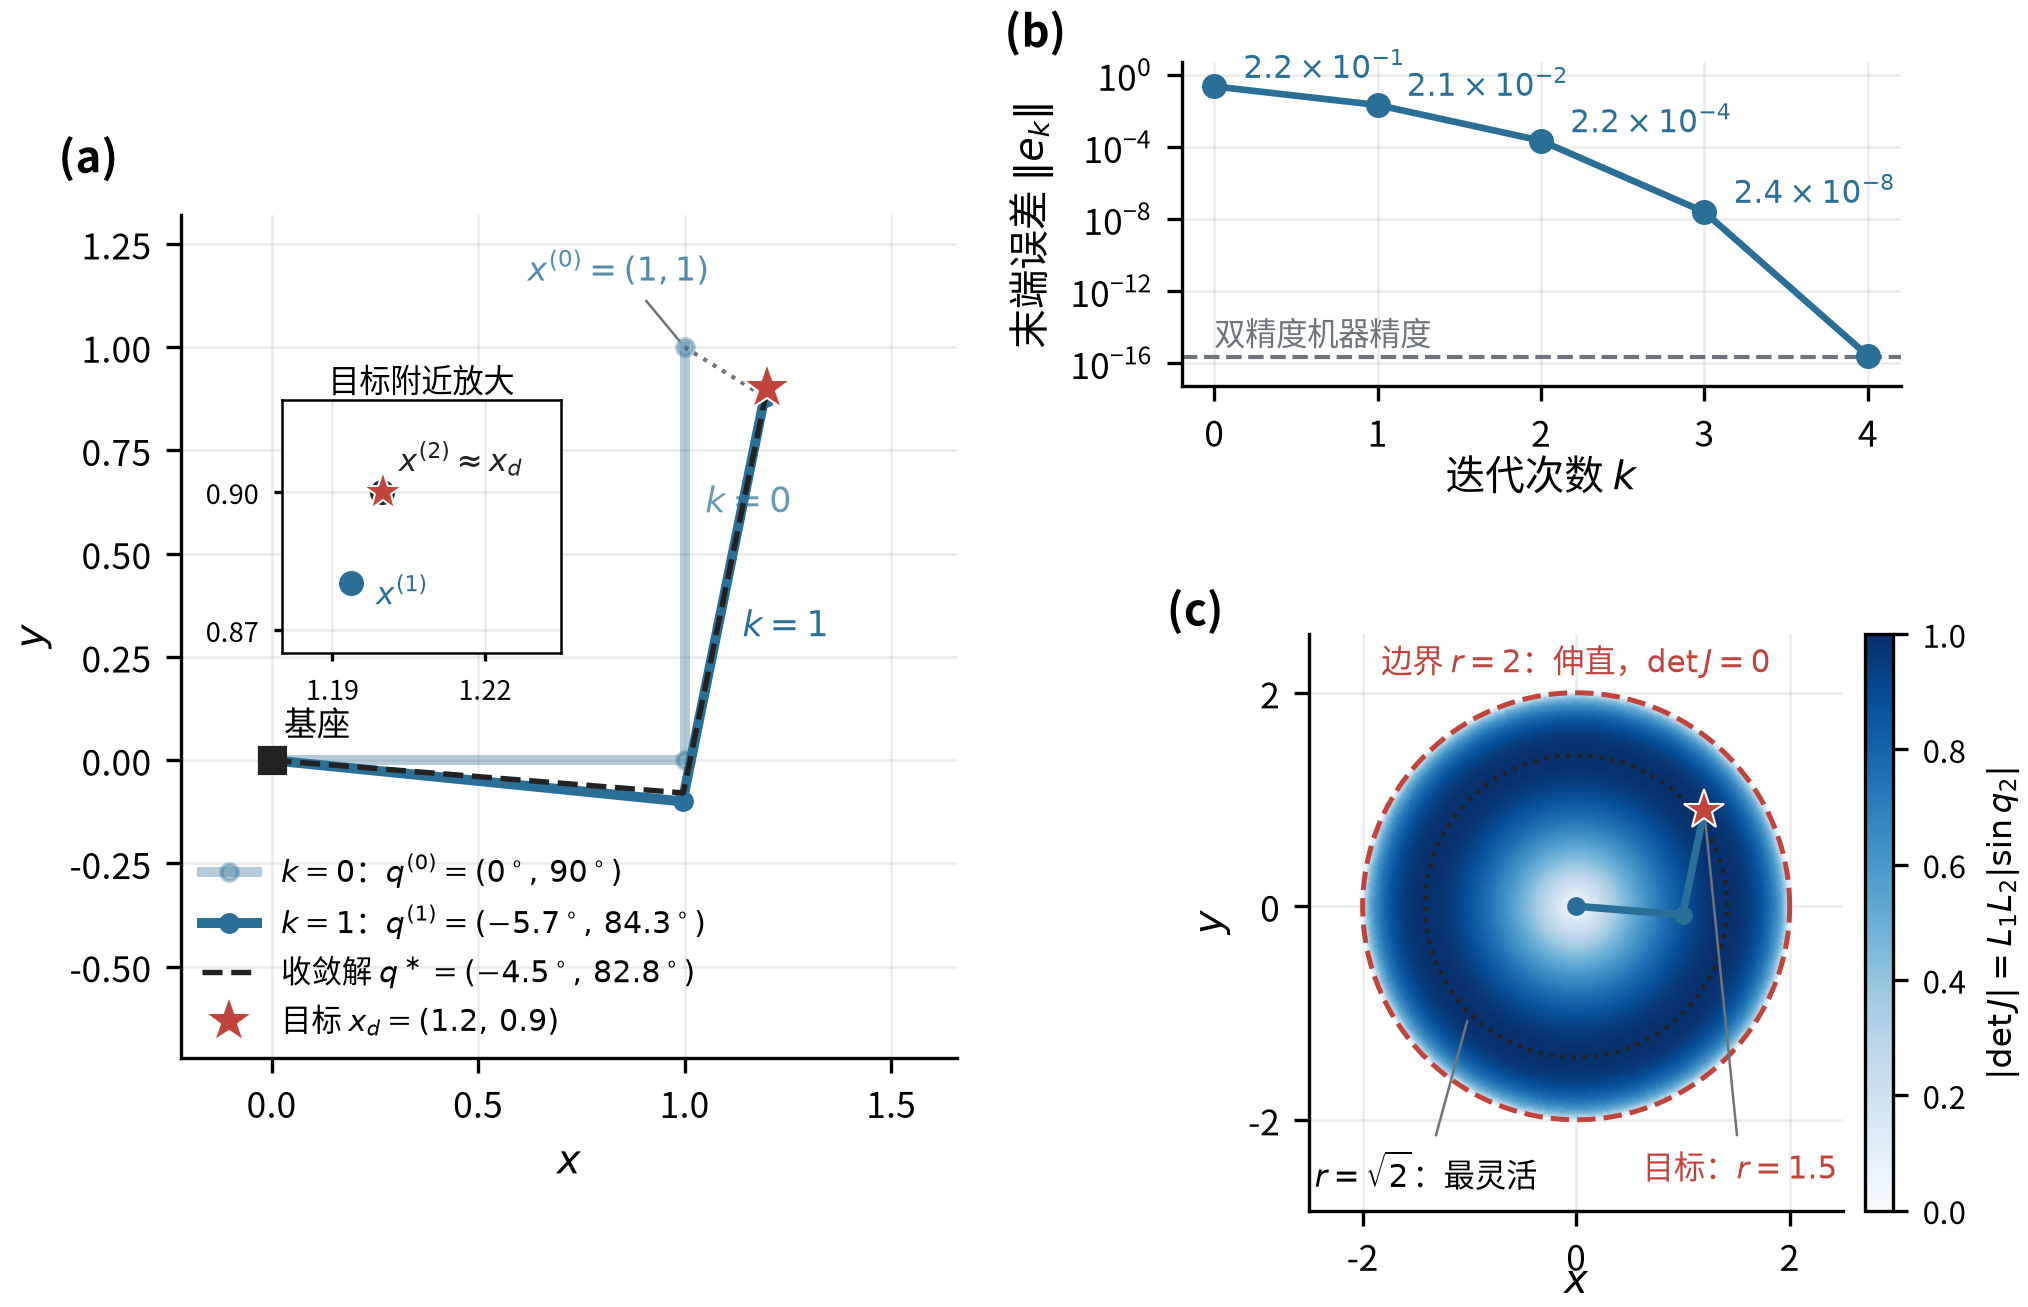
\includegraphics[width=0.98\textwidth]{figures/chap06/chap06_fig1.png}
\caption{牛顿迭代法求解逆运动学：与上面手算示例相同的设定（$L_1 = L_2 = 1$，目标 $x_d = (1.2,\,0.9)$，初值 $q^{(0)} = (0^\circ, 90^\circ)$），由 \texttt{code/chap07\_robotics.py} 实际迭代得到。（a）迭代过程中的机械臂姿态：一步之后末端到目标的距离已从 $0.22$ 缩到 $0.02$，两步之后与收敛解 $q^\ast = (-4.5^\circ,\,82.8^\circ)$ 肉眼已不可分（插图放大了目标附近）。（b）末端误差 $\|e_k\| = \|x_d - f(q^{(k)})\|$ 随迭代次数的变化（对数轴）：$2\times10^{-1} \to 2\times10^{-2} \to 2\times10^{-4} \to 2\times10^{-8}$，误差的指数每步大约翻一倍——这就是牛顿法的二次收敛，四步即达双精度机器精度。（c）工作空间上的可操作度 $|\det J| = L_1 L_2 |\sin q_2|$：外圈 $r = 2$（手臂伸直）与圆心是奇异位形，$r = \sqrt{2}$（$q_2 = 90^\circ$）处最灵活；目标点在 $r = 1.5$，离奇异位形很远，$J$ 良态，所以牛顿法收敛得又快又稳。}
\label{fig:chap06_robotics}
\end{figure}

\paragraph{当雅可比不可逆时怎么办？}

如果 $n > m$（冗余机械臂，$J$ 不是方阵），$J$ 没有逆。这时用\textbf{伪逆}（要求 $J$ 行满秩）：

\[
\Delta q = J^\dagger e, \quad \text{其中 } J^\dagger = J^\top(JJ^\top)^{-1}
\]

伪逆给出的是\textbf{最小范数解}——在所有能消除误差的 $\Delta q$ 中，选择最小的那个。在奇异位形附近 $JJ^\top$ 接近奇异，伪逆会“爆炸”，实践中改用阻尼最小二乘 $J^\top(JJ^\top + \delta^2 I)^{-1}$（习题 8）。
\clarify{伪逆不是“另一种方法”，它就是上一小节 KKT 条件的解：$\min \tfrac{1}{2}\|\Delta q\|^2$ s.t. $J\Delta q = e$ 给出 $\Delta q = -J^\top \lambda$，代回约束得 $\lambda = -(JJ^\top)^{-1} e$，于是 $\Delta q = J^\dagger e$。“最小范数解” = 拉格朗日乘子法的解。}

\begin{example}[几何解法 vs 迭代解法]
双连杆机械臂，$L_1 = L_2 = 1$，目标位置 $(1.0, 1.0)$。

\textbf{几何解法}（利用特殊结构）：

由于连杆等长，可以用余弦定理直接求解。

设末端到原点的距离为 $r = \sqrt{1^2 + 1^2} = \sqrt{2}$。

\begin{figure}[htbp]
\centering
\begin{tikzpicture}[scale=1.5]
    % 坐标系
    \draw[->] (-0.3,0) -- (1.8,0) node[right] {$x$};
    \draw[->] (0,-0.3) -- (0,1.8) node[above] {$y$};
    
    % 两种解
    % 解1：手肘朝上
    \draw[very thick, blue] (0,0) -- (0,1) -- (1,1);
    \fill[blue] (0,1) circle (2pt) node[left] {\small 肘};
    
    % 解2：手肘朝下（虚线）
    \draw[thick, blue, dashed] (0,0) -- (1,0) -- (1,1);
    \fill[blue, opacity=0.5] (1,0) circle (2pt) node[below] {\small 肘};
    
    % 目标点
    \fill[red] (1,1) circle (3pt) node[above right] {$(1,1)$};
    
    % 原点
    \fill (0,0) circle (2pt) node[below left] {$O$};
    
    % 距离标注
    \draw[<->, gray] (0.1,0.1) -- (0.9,0.9);
    \node[gray] at (0.7,0.3) {$r=\sqrt{2}$};
\end{tikzpicture}
\caption{逆运动学的两个解：手肘朝上或朝下}
\end{figure}

在三角形中，由余弦定理：
\[
r^2 = L_1^2 + L_2^2 - 2L_1 L_2 \cos(\pi - q_2)
\]

注意 $\pi - q_2$ 是三角形的内角，而 $q_2$ 是肘关节的弯曲角度。

代入数值：
\[
2 = 1 + 1 + 2 \cdot 1 \cdot 1 \cdot \cos q_2 \quad \Rightarrow \quad \cos q_2 = 0 \quad \Rightarrow \quad q_2 = \pm 90°
\]

于是有两个解：$q_2 = +90°$ 对应手肘朝上（图中实线），$q_2 = -90°$ 对应手肘朝下（图中虚线）。

取 $q_2 = 90°$，代入正运动学方程求 $q_1$：
\begin{align}
1 &= \cos q_1 + \cos(q_1 + 90°) = \cos q_1 - \sin q_1 \\
1 &= \sin q_1 + \sin(q_1 + 90°) = \sin q_1 + \cos q_1
\end{align}

两式相加：$2 = 2\cos q_1$，所以 $\cos q_1 = 1$，$q_1 = 0°$。

\textbf{验证}：
\[
x = \cos 0° + \cos 90° = 1 + 0 = 1 \quad \checkmark
\]
\[
y = \sin 0° + \sin 90° = 0 + 1 = 1 \quad \checkmark
\]

\textbf{总结}：几何解法快速直接，但只适用于简单结构。牛顿迭代法适用于任意复杂的机械臂。
\end{example}

\subsection{冗余机械臂与零空间}

\paragraph{什么是冗余？}

当机械臂的关节数 $n$ 大于任务空间维度 $m$ 时，我们说它是\textbf{冗余}的。

\begin{center}
\renewcommand{\arraystretch}{1.3}
\begin{tabular}{l|c|c|l}
\toprule
\textbf{例子} & \textbf{关节数 $n$} & \textbf{任务维度 $m$} & \textbf{冗余度 $n-m$} \\
\midrule
平面双连杆 & 2 & 2 & 0（恰好） \\
典型工业臂 & 6 & 6 & 0（恰好） \\
人的手臂 & 7 & 6 & 1 \\
双臂机器人 & 14 & 6（单手任务） & 8 \\
蛇形机器人 & 20+ & 6 & 14+ \\
\bottomrule
\end{tabular}
\end{center}

\paragraph{冗余意味着什么？}

冗余意味着逆运动学有\textbf{无穷多解}。直觉上：完成同一个任务，有很多种姿势可以选择。

\begin{example}[人手臂的冗余]
做一个实验：把你的手掌放在桌面上固定不动，然后在保持手掌位置和朝向不变的前提下移动你的手肘。你会发现，手肘可以在一个弧线上移动，而手掌完全不动——这就是冗余带来的自由度。正是这个“额外”的自由度，让我们能在狭窄空间里绕开障碍物、避免撞到自己的身体，或者干脆换一个更舒服的姿势。
\end{example}

\paragraph{零空间的数学描述}\mbox{}\par\nopagebreak

\begin{definition}[零空间]
雅可比矩阵 $J$ 的\textbf{零空间}（Null Space）是所有满足 $J v = 0$ 的向量 $v$ 的集合：
\[
\mathcal{N}(J) = \{ v \in \mathbb{R}^n : Jv = 0 \}
\]
\end{definition}

\textbf{物理意义}：如果关节速度 $\dot{q}$ 在零空间中，那么 $\dot{x} = J\dot{q} = 0$——末端不动！

换句话说，零空间运动是“内部运动”——关节在动，但末端静止。

\begin{figure}[htbp]
\centering
\begin{tikzpicture}[scale=1.0]
    % 左图：三连杆机械臂，两种构型
    \begin{scope}[shift={(0,0)}]
        \node at (2,-2) {\textbf{(a) 三连杆机械臂}};
        
        % 构型1
        \draw[very thick, blue] (0,0) -- (1,1.5) -- (2.5,1.8) -- (3.5,1);
        \fill (0,0) circle (2pt);
        \fill (1,1.5) circle (2pt);
        \fill (2.5,1.8) circle (2pt);
        \fill[red] (3.5,1) circle (3pt);
        
        % 构型2（虚线）
        \draw[thick, blue, dashed] (0,0) -- (1.5,0.8) -- (2.8,1.5) -- (3.5,1);
        \fill[blue, opacity=0.3] (1.5,0.8) circle (2pt);
        \fill[blue, opacity=0.3] (2.8,1.5) circle (2pt);
        
        % 说明
        \node[red] at (3.5,0.5) {\small 末端固定};
        \draw[<->, dashed, gray] (1,1.5) .. controls (1.3,1.1) .. (1.5,0.8);
        \node[gray] at (0.5,1) {\scriptsize 零空间运动};
    \end{scope}
    
    % 右图：零空间示意
    \begin{scope}[shift={(7,0)}]
        \node at (2,-2) {\textbf{(b) 零空间示意}};
        
        % 关节空间
        \draw[->] (0,0) -- (3.5,0) node[right] {$\dot{q}_1$};
        \draw[->] (0,0) -- (0,2.5) node[above] {$\dot{q}_2$};
        
        % 零空间（一条线）
        \draw[very thick, green!60!black] (-0.5,-0.3) -- (3,1.8);
        \node[green!60!black] at (3.2,2) {$\mathcal{N}(J)$};
        
        % 一个向量
        \draw[->, thick, blue] (0,0) -- (2,1.2);
        \node[blue] at (1.5,0.5) {$\dot{q} \in \mathcal{N}(J)$};
        
        % 说明
        \node at (1.5,-0.8) {\small 沿此方向运动};
        \node at (1.5,-1.2) {\small 末端速度为零};
    \end{scope}
\end{tikzpicture}
\caption{零空间运动：关节在动，末端不动}
\end{figure}

\paragraph{冗余逆运动学的通解}

当 $n > m$ 时，逆运动学的解可以写成：

\begin{keyformula}[title=冗余逆运动学的通解]
\begin{equation}
\dot{q} = \underbrace{J^\dagger \dot{x}_d}_{\text{完成主任务}} + \underbrace{(I - J^\dagger J) z}_{\text{零空间运动}}
\end{equation}
其中 $J^\dagger = J^\top(JJ^\top)^{-1}$ 是\textbf{伪逆}，$\dot{x}_d$ 是期望的末端速度，$(I - J^\dagger J)$ 是\textbf{零空间投影矩阵}，而 $z \in \mathbb{R}^n$ 是\textbf{任意向量}。
\end{keyformula}

\begin{physicalmeaning}
这个公式把关节速度拆成了两部分。第一项 $J^\dagger \dot{x}_d$ 保证末端以期望速度 $\dot{x}_d$ 运动；第二项 $(I - J^\dagger J) z$ 落在零空间中，所以无论 $z$ 取什么，它都不影响末端。于是 $z$ 可以自由选择，用来实现\textbf{次级目标}。
\end{physicalmeaning}

\paragraph{次级目标的例子}

$z$ 可以怎么选？常见的做法是取某个标量函数的梯度，让零空间运动顺着它上升或下降。若想\textbf{远离关节限位}，可取
\[
z = -k \nabla_q W(q), \quad W(q) = \sum_i \frac{1}{(q_i - q_i^{min})(q_i^{max} - q_i)}
\]
$W$ 在关节接近限位时变大，负梯度方向指向“远离限位”。若想\textbf{避开障碍物}，可取 $z = k \nabla_q d(q)$，其中 $d(q)$ 是机械臂与障碍物的最近距离，沿梯度方向走就是把距离拉大。若想\textbf{最小化能量}，则取 $z = -k \nabla_q \|\tau\|^2$，让关节力矩尽可能小。

\begin{example}[冗余的实际应用]
想象一个7自由度机械臂在一个有障碍物的环境中工作：

\begin{figure}[htbp]
\centering
\begin{tikzpicture}[scale=0.9]
    % 障碍物
    \fill[gray!40] (2,0.5) rectangle (2.5,2);
    \node at (2.25,2.3) {\small 障碍物};
    
    % 构型1：会撞到障碍物
    \draw[thick, red, dashed] (0,0) -- (1,1) -- (2.2,1.2) -- (3.5,0.8);
    \fill[red, opacity=0.5] (2.2,1.2) circle (3pt);
    \node[red] at (1.5,1.5) {\small 碰撞！};
    
    % 构型2：绕开障碍物
    \draw[very thick, blue] (0,0) -- (0.8,1.5) -- (1.5,2.2) -- (3.5,0.8);
    \fill (0,0) circle (2pt);
    \fill (0.8,1.5) circle (2pt);
    \fill (1.5,2.2) circle (2pt) node[above] {\small 肘抬高};
    \fill[red] (3.5,0.8) circle (3pt) node[right] {\small 末端};
    
    % 说明
    \node at (1.75,-0.5) {\small 利用零空间绕开障碍物};
\end{tikzpicture}
\caption{冗余自由度让机械臂能够在保持末端位置的同时避开障碍物}
\end{figure}

两种构型的末端位置相同，但只有蓝色构型能避开障碍物。冗余自由度提供了这种灵活性。
\end{example}
\preview{第7章会把“选一个 $z$ 做次级目标”升级为对整条轨迹 $q(t)$ 做优化：动力学约束用拉格朗日乘子（伴随变量）处理，这就是轨迹优化和 MPC。}

% ------------------------------------------------------------------------------------
\section{机器人动力学：力与运动的关系}

\subsection{为什么需要动力学？}

到目前为止，我们讨论的运动学只关心\textbf{几何关系}——关节角度和末端位置的对应。但实际控制机器人时，我们需要知道：

\begin{quote}
\textit{电机应该输出多大的力矩，才能让机械臂按照期望的方式运动？}
\end{quote}

这就是\textbf{动力学}要回答的问题。

\begin{example}[直觉理解]
想象你在举哑铃。哑铃越重，举起它需要的力越大，这是质量的作用；想举得越快，需要的力也越大，这是加速度的作用；即使哑铃静止不动，你也得持续用力来抵抗重力；而如果哑铃在转动，你还会感到一些“奇怪”的力——科氏力和离心力。机器人动力学就是要把这些直觉变成精确的数学公式。
\end{example}

\subsection{复习：拉格朗日方程}

在第5章，我们学过拉格朗日方程：
\begin{equation}
\frac{d}{dt}\frac{\partial L}{\partial \dot{q}_i} - \frac{\partial L}{\partial q_i} = Q_i
\end{equation}

其中 $L = T - V$ 是拉格朗日量（动能减势能），$q_i$ 是广义坐标，对机器人来说就是关节角度，$Q_i$ 是广义力，对机器人来说就是关节力矩 $\tau_i$。

这个方程的美妙之处在于：只要写出动能和势能的表达式，力学方程就自动出来了！
\clarify{第5章的拉格朗日方程右边是 0，广义力 $F_i = \partial L/\partial q_i$ 指的是保守力（势能的负梯度）。这里右边的 $Q_i$ 是电机、摩擦这类不能写进势能的外力——它们必须单独加在右边。}

\subsection{机器人的动能}

\paragraph{单连杆的动能}

考虑一根绕端点转动的杆（单摆），质量 $m$，长度 $L$，假设质量集中在末端：

\begin{figure}[htbp]
\centering
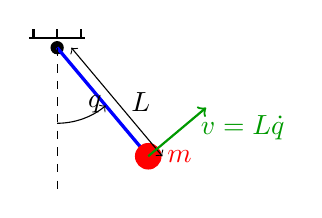
\begin{tikzpicture}[scale=1.2]
    % 固定点
    \fill (0,0) circle (2pt);
    \draw[thick] (-0.3,0.1) -- (0.3,0.1);
    \draw[thick] (-0.25,0.1) -- (-0.25,0.2);
    \draw[thick] (0,0.1) -- (0,0.2);
    \draw[thick] (0.25,0.1) -- (0.25,0.2);
    
    % 连杆
    \draw[very thick, blue] (0,0) -- ({1.5*sin(40)},{-1.5*cos(40)});
    
    % 质点
    \fill[red] ({1.5*sin(40)},{-1.5*cos(40)}) circle (4pt);
    \node[red, right] at ({1.5*sin(40)+0.1},{-1.5*cos(40)}) {$m$};
    
    % 角度
    \draw[dashed] (0,0) -- (0,-1.5);
    \draw[->] (0,-0.8) arc (-90:-50:0.8);
    \node at (0.4,-0.6) {$q$};
    
    % 长度
    \draw[<->] (0.15,0) -- ({1.5*sin(40)+0.15},{-1.5*cos(40)});
    \node[right] at ({0.75*sin(40)+0.2},{-0.75*cos(40)}) {$L$};
    
    % 速度
    \draw[->, thick, green!60!black] ({1.5*sin(40)},{-1.5*cos(40)}) -- 
        ({1.5*sin(40)+0.8*cos(40)},{-1.5*cos(40)+0.8*sin(40)});
    \node[green!60!black] at ({1.5*sin(40)+1},{-1.5*cos(40)+0.3}) {$v = L\dot{q}$};
\end{tikzpicture}
\caption{单摆：最简单的“机器人”}
\end{figure}

质点的速度大小为 $v = L\dot{q}$（圆周运动），所以动能是：
\begin{equation}
T = \frac{1}{2}mv^2 = \frac{1}{2}m(L\dot{q})^2 = \frac{1}{2}mL^2 \dot{q}^2
\end{equation}

我们可以定义\textbf{转动惯量} $I = mL^2$，则 $T = \frac{1}{2}I\dot{q}^2$。

\paragraph{多连杆的动能}

对于多连杆机械臂，每个连杆都在运动，总动能是各部分之和。关键观察是：每个连杆的速度取决于\textbf{所有它之前的关节}的角度和角速度。

最终，总动能可以写成：
\begin{equation}
T = \frac{1}{2} \dot{q}^\top M(q) \dot{q}
\end{equation}

其中 $M(q)$ 是 $n \times n$ 的\textbf{质量矩阵}（也叫惯性矩阵）。

\begin{physicalmeaning}
$M(q)$ 的每个元素都有物理意义：对角元 $M_{ii}$ 是第 $i$ 个关节单独转动时的“有效惯量”，非对角元 $M_{ij}$（$i \neq j$）是关节 $i$ 和 $j$ 之间的“惯性耦合”。整个矩阵依赖于位形 $q$——机械臂伸直时和弯曲时，惯量不同！
\end{physicalmeaning}

\begin{example}[伸直 vs 弯曲的惯量]
想象一根双连杆机械臂：

\begin{figure}[htbp]
\centering
\begin{tikzpicture}[scale=1.0]
    % 伸直
    \begin{scope}[shift={(0,0)}]
        \draw[very thick, blue] (0,0) -- (2,0) -- (4,0);
        \fill (0,0) circle (2pt);
        \fill (2,0) circle (2pt);
        \fill[red] (4,0) circle (3pt);
        \draw[->] (0,-0.5) arc (-90:0:0.5);
        \node at (0.7,-0.3) {$\dot{q}_1$};
        \node at (2,-1) {\small 伸直：转动惯量大};
    \end{scope}
    
    % 弯曲
    \begin{scope}[shift={(6,0)}]
        \draw[very thick, blue] (0,0) -- (1.5,0) -- (1.5,-1.5);
        \fill (0,0) circle (2pt);
        \fill (1.5,0) circle (2pt);
        \fill[red] (1.5,-1.5) circle (3pt);
        \draw[->] (0,-0.5) arc (-90:0:0.5);
        \node at (0.7,-0.3) {$\dot{q}_1$};
        \node at (1,-2) {\small 弯曲：转动惯量小};
    \end{scope}
\end{tikzpicture}
\caption{质量矩阵依赖于位形}
\end{figure}

当手臂伸直时，末端离肩关节很远，绕肩关节转动时需要更大的力矩。这体现在 $M_{11}$ 更大。

当手臂弯曲时，末端离肩关节近，转动惯量变小。
\end{example}

\subsection{机器人的势能}

对于大多数机器人，势能只来自重力：
\begin{equation}
V = \sum_i m_i g h_i(q)
\end{equation}

其中 $h_i(q)$ 是第 $i$ 个连杆质心的高度（取决于关节角度 $q$）。

\subsection{推导动力学方程}

现在让我们用拉格朗日方程推导机器人的动力学。

\paragraph{第一步：计算 $\frac{\partial L}{\partial \dot{q}}$}

\begin{align}
\frac{\partial L}{\partial \dot{q}} &= \frac{\partial T}{\partial \dot{q}} - \frac{\partial V}{\partial \dot{q}} \\
&= \frac{\partial}{\partial \dot{q}} \left( \frac{1}{2} \dot{q}^\top M(q) \dot{q} \right) - 0 \\
&= M(q) \dot{q}
\end{align}

（这里用到了 $\frac{\partial}{\partial x}(x^\top A x) = 2Ax$ 对于对称矩阵 $A$。）

\paragraph{第二步：计算 $\frac{d}{dt}\frac{\partial L}{\partial \dot{q}}$}

\begin{align}
\frac{d}{dt}(M(q)\dot{q}) &= \dot{M}(q)\dot{q} + M(q)\ddot{q}
\end{align}

这里 $\dot{M}$ 是 $M$ 对时间的导数，它依赖于 $\dot{q}$。

\paragraph{第三步：计算 $\frac{\partial L}{\partial q}$}

\begin{align}
\frac{\partial L}{\partial q} &= \frac{\partial T}{\partial q} - \frac{\partial V}{\partial q}
\end{align}

$\frac{\partial T}{\partial q}$ 来自 $M(q)$ 对 $q$ 的依赖，$\frac{\partial V}{\partial q}$ 是重力产生的力。

\paragraph{第四步：整理}

把所有项放在一起，经过仔细整理（具体推导需要一些技巧），最终得到：

\begin{keyformula}[title=机器人动力学标准形式]
\begin{equation}
\boxed{M(q)\ddot{q} + C(q, \dot{q})\dot{q} + G(q) = \tau}
\end{equation}
\end{keyformula}

\begin{center}
\renewcommand{\arraystretch}{1.5}
\begin{tabular}{c|l|p{7cm}}
\toprule
\textbf{符号} & \textbf{名称} & \textbf{物理意义} \\
\midrule
$M(q)\ddot{q}$ & 惯性项 & 加速关节需要的力矩，就像 $F = ma$ \\
$C(q, \dot{q})\dot{q}$ & 科氏力/离心力 & 速度引起的“假想力”，旋转坐标系中才有 \\
$G(q)$ & 重力项 & 抵抗重力需要的力矩 \\
$\tau$ & 关节力矩 & 电机需要输出的力矩 \\
\bottomrule
\end{tabular}
\end{center}

\begin{example}[单摆的完整推导]
让我们对单摆完整做一遍拉格朗日推导。

\textbf{设置}：质量 $m$，长度 $L$，关节角 $q$（从竖直向下测量）。

\textbf{动能}：
\[
T = \frac{1}{2}mL^2\dot{q}^2
\]

\textbf{势能}（以铰链为零势能点）：
\[
V = -mgL\cos q
\]

注意：当 $q = 0$（竖直向下）时，$V = -mgL$（最低）；当 $q = 90°$（水平）时，$V = 0$。

\textbf{拉格朗日量}：
\[
L = T - V = \frac{1}{2}mL^2\dot{q}^2 + mgL\cos q
\]

\textbf{计算各项}：
\begin{align}
\frac{\partial L}{\partial \dot{q}} &= mL^2\dot{q} \\
\frac{d}{dt}\frac{\partial L}{\partial \dot{q}} &= mL^2\ddot{q} \\
\frac{\partial L}{\partial q} &= -mgL\sin q
\end{align}

\textbf{拉格朗日方程}：
\[
mL^2\ddot{q} - (-mgL\sin q) = \tau
\]

即：
\[
\boxed{mL^2\ddot{q} + mgL\sin q = \tau}
\]

\textbf{对比标准形式}：$M = mL^2$ 是常数，因为单摆只有一个关节；$C = 0$，单关节没有科氏力；$G = mgL\sin q$ 是重力产生的力矩。

\textbf{物理检验}：当 $q = 0$（竖直向下）时 $G = 0$，不需要力矩来维持；当 $q = 90°$（水平）时 $G = mgL$，需要的力矩最大；当 $q = 180°$（竖直向上）时 $G$ 又回到 0，但这是不稳定平衡。
\end{example}

\begin{example}[双连杆机械臂的动力学（概念性）]
对于双连杆机械臂，动力学方程会更复杂。质量矩阵是 $2 \times 2$：

\[
M(q) = \begin{bmatrix}
M_{11}(q_2) & M_{12}(q_2) \\
M_{12}(q_2) & M_{22}
\end{bmatrix}
\]

这里 $M_{11}$ 依赖于肘关节角度 $q_2$：手臂弯曲时，肩关节的有效惯量变小；$M_{22}$ 是常数，肘关节的惯量不受其他关节影响；而 $M_{12} = M_{21}$，这个对称性来自动能的二次型性质。

科氏力矩阵 $C$ 包含 $\dot{q}_1^2$ 和 $\dot{q}_1\dot{q}_2$ 等项——这些是快速运动时产生的“假想力”。

重力向量 $G$ 包含 $\sin$ 和 $\cos$ 项——取决于各连杆的角度。

具体表达式很长，通常用符号计算软件导出。
\end{example}

\subsection{动力学的重要性质}

机器人动力学有几个重要的数学性质，它们对控制设计很有用：

\paragraph{性质1：质量矩阵对称正定}
\[
M(q) = M(q)^\top, \quad M(q) > 0
\]

\textbf{物理意义}：动能 $T = \frac{1}{2}\dot{q}^\top M \dot{q}$ 总是正的（只要有运动）。

\paragraph{性质2：$\dot{M} - 2C$ 反对称}
\[
\dot{q}^\top (\dot{M} - 2C) \dot{q} = 0
\]

\textbf{物理意义}：这保证了能量守恒。如果没有外力（$\tau = 0$）且忽略重力，系统能量 $T$ 保持不变。

\begin{proof}[简单说明]
对动能求时间导数：
\begin{align}
\frac{dT}{dt} &= \frac{d}{dt}\left(\frac{1}{2}\dot{q}^\top M \dot{q}\right) \\
&= \frac{1}{2}\dot{q}^\top \dot{M} \dot{q} + \dot{q}^\top M \ddot{q}
\end{align}

把 $M\ddot{q} = \tau - C\dot{q} - G$ 代入：
\begin{align}
\frac{dT}{dt} &= \frac{1}{2}\dot{q}^\top \dot{M} \dot{q} + \dot{q}^\top (\tau - C\dot{q} - G) \\
&= \dot{q}^\top \tau - \dot{q}^\top G + \frac{1}{2}\dot{q}^\top (\dot{M} - 2C) \dot{q}
\end{align}

如果 $\dot{M} - 2C$ 反对称，最后一项为零，于是：
\[
\frac{dT}{dt} = \dot{q}^\top \tau - \dot{q}^\top G = \text{功率输入} - \text{重力功率}
\]

这正是能量守恒的表达！
\end{proof}

\paragraph{性质3：线性于参数}

动力学方程可以写成：
\[
M(q)\ddot{q} + C(q,\dot{q})\dot{q} + G(q) = Y(q, \dot{q}, \ddot{q}) \theta
\]

其中 $Y$ 是已知的矩阵（只依赖于运动状态），$\theta$ 是物理参数向量（质量、惯量、质心位置等）。

\textbf{应用}：这个性质让我们能够通过测量运动和力矩来\textbf{辨识}机器人的物理参数。

% ------------------------------------------------------------------------------------
\section{接触力学：当机器人碰到东西时}

\subsection{为什么接触很重要？}

机器人与世界交互几乎总是通过接触：机械臂抓取物体、腿式机器人行走、工业机器人装配零件、手术机器人操作组织，无一例外。没有接触力的分析，我们无法理解机器人如何真正“做事”。

\begin{example}[行走的秘密]
当你走路时，脚蹬地，地面给你一个向前的摩擦力，推动你前进。

如果地面是完美光滑的（没有摩擦），你只能原地踏步——就像在冰面上一样。

机器人行走也是如此：地面反作用力是推动机器人前进的“动力来源”。
\end{example}

\subsection{接触力如何进入动力学方程}

当机器人与环境接触时，接触点受到\textbf{接触力} $\lambda_c$。这个力如何影响关节运动？

答案是通过\textbf{雅可比转置}——和末端力传递完全一样！

\begin{keyformula}[title=带接触的动力学方程]
\begin{equation}
M(q)\ddot{q} + C(q,\dot{q})\dot{q} + G(q) = \tau + J_c(q)^\top \lambda_c
\end{equation}

其中 $J_c(q)$ 是接触点的雅可比矩阵，$\lambda_c$ 是作用在接触点处的接触力，$J_c^\top \lambda_c$ 则是接触力在关节空间产生的\textbf{广义力}。
\end{keyformula}

\begin{keyformula}[title=接触动力学的 KKT 形式]
保持接触时 $\phi(q) \equiv 0$，对时间求两次导得 $J_c \ddot{q} + \dot{J}_c \dot{q} = 0$。把它和动力学方程并起来：
\begin{equation}
\begin{bmatrix} M(q) & -J_c^\top \\ J_c & 0 \end{bmatrix}
\begin{bmatrix} \ddot{q} \\ \lambda_c \end{bmatrix}
=
\begin{bmatrix} \tau - C\dot{q} - G \\ -\dot{J}_c \dot{q} \end{bmatrix}
\end{equation}
对比第1章的 KKT 矩阵 $\begin{bmatrix} \nabla^2_{xx}\Lag & (\nabla g)^\top \\ \nabla g & 0 \end{bmatrix}$（符号约定不同，结构相同）：质量矩阵 $M$ 扮演 Hessian，约束雅可比 $J_c$ 扮演 $\nabla g$，接触力 $\lambda_c$ 就是乘子。这正是“高斯最小拘束原理”：在所有满足接触约束的加速度中，真实的 $\ddot{q}$ 使 $\tfrac{1}{2}(\ddot{q} - \ddot{q}_{\text{free}})^\top M (\ddot{q} - \ddot{q}_{\text{free}})$ 最小（$\ddot{q}_{\text{free}} = M^{-1}(\tau - C\dot{q} - G)$ 是无接触时的加速度），$\lambda_c$ 是这个二次规划的乘子。
\end{keyformula}
\review{第1章}{第1章扩展阅读预告过：KKT 矩阵会在本章以“质量矩阵 + 约束雅可比”的形式出现——就是上面这个分块矩阵。第1章思考题 9 的答案也在这里：$H \leftrightarrow M$，$\nabla g \leftrightarrow J_c$，$\lambda \leftrightarrow$ 接触力。}

\begin{physicalmeaning}
$J_c^\top$ 把接触点的力“传递”到关节空间，就像 $J^\top$ 把末端力传递到关节一样。

这正是我们在约束优化中见过的\textbf{拉格朗日乘子}！$\lambda_c$ 是接触约束的乘子，它自动给出了维持约束所需的力。
\end{physicalmeaning}

\subsection{接触力的物理约束}

接触力不是任意的，它必须满足物理约束：

\paragraph{约束1：不能穿透}

设 $\phi(q)$ 是接触间隙，即机器人与环境之间的最近距离：$\phi > 0$ 表示没有接触，$\phi = 0$ 表示正在接触，而 $\phi < 0$ 意味着穿透，物理上不允许。于是约束是 $\phi(q) \geq 0$。

\paragraph{约束2：法向力是推力}

接触面只能“推”不能“拉”（除非有吸盘）：
\[
\lambda_n \geq 0
\]

其中 $\lambda_n$ 是法向接触力。

\paragraph{约束3：互补松弛}

这是最关键的条件：
\[
\lambda_n \cdot \phi(q) = 0
\]

它的含义是两者至少有一个为零：如果 $\phi > 0$（不接触），则 $\lambda_n = 0$（没有力）；反过来，如果 $\lambda_n > 0$（有力），则必有 $\phi = 0$（正在接触）。

\begin{figure}[htbp]
\centering
\begin{tikzpicture}[scale=1.4]
    % 地面
    \fill[gray!20] (-0.5,-0.1) rectangle (8,0);
    \draw[thick] (-0.5,0) -- (8,0);
    
    % 状态1：悬空
    \begin{scope}[shift={(1,0)}]
        \draw[thick, blue, fill=blue!20] (0,1) circle (0.4);
        \node at (0,1) {\small 球};
        \draw[->, red, thick] (0,0.6) -- (0,0.15) node[right] {$mg$};
        
        \node at (0,-0.4) {\small $\phi > 0$};
        \node at (0,-0.7) {\small $\lambda = 0$};
        \node at (0,1.7) {\small \textbf{悬空}};
    \end{scope}
    
    % 状态2：静止接触
    \begin{scope}[shift={(3.5,0)}]
        \draw[thick, blue, fill=blue!20] (0,0.4) circle (0.4);
        \node at (0,0.4) {\small 球};
        \draw[->, red, thick] (0,0.4) -- (0,-0.25) node[right] {$mg$};
        \draw[->, green!60!black, thick] (0,0) -- (0,0.65) node[left] {$\lambda$};
        
        \node at (0,-0.4) {\small $\phi = 0$};
        \node at (0,-0.7) {\small $\lambda = mg$};
        \node at (0,1.1) {\small \textbf{静止接触}};
    \end{scope}
    
    % 状态3：滑动接触
    \begin{scope}[shift={(6,0)}]
        \draw[thick, blue, fill=blue!20] (0,0.4) circle (0.4);
        \node at (0,0.4) {\small 球};
        \draw[->, red, thick] (0,0.4) -- (0,-0.25);
        \draw[->, green!60!black, thick] (0,0) -- (0,0.65);
        \draw[->, orange, thick] (0,0) -- (0.5,0) node[above] {$f$};
        \draw[->, blue, thick] (0.4,0.4) -- (0.9,0.4) node[above] {$v$};
        
        \node at (0,-0.4) {\small $\phi = 0$};
        \node at (0,-0.7) {\small $|f| = \mu\lambda$};
        \node at (0,1.1) {\small \textbf{滑动接触}};
    \end{scope}
\end{tikzpicture}
\caption{接触的三种状态}
\end{figure}

\begin{insightbox}
互补松弛条件 $\lambda \cdot \phi = 0$ 和第2章线性规划中的互补松弛完全一样！

在线性规划中：“免费的资源没人用，稀缺的资源才有价格”。

在接触力学中：“悬空时没有力，接触时才有力”。

这是同一个数学结构在不同领域的体现。
\end{insightbox}
\review{第2章}{第2章的互补松弛：对偶变量 $y_i$ 和松弛量 $s_i$ 至少一个为零——“免费的资源没人用，稀缺的资源才有价格”。把 $y_i$ 换成 $\lambda_n$、$s_i$ 换成间隙 $\phi$，就是这里的条件。}

\subsection{摩擦力与库仑锥}

除了法向力，接触通常还有\textbf{摩擦力}（切向力）。

\paragraph{库仑摩擦模型}

最常用的摩擦模型是库仑模型。它区分两种情形：物体静止时是静摩擦，摩擦力可以指向任意方向，但大小受限；物体滑动时是动摩擦，摩擦力与速度方向相反，大小正比于法向力。两种情形合起来写成一个不等式：
\[
\|f_t\| \leq \mu \lambda_n
\]

其中 $f_t$ 是切向力，$\mu$ 是摩擦系数，$\lambda_n$ 是法向力。

\paragraph{摩擦锥}

这个不等式定义了一个\textbf{锥形区域}：接触力必须在锥内。

\begin{figure}[htbp]
\centering
\begin{tikzpicture}[scale=1.2]
    % 三维摩擦锥
    \begin{scope}[shift={(0,0)}]
        % 底面（椭圆表示圆）
        \draw[thick, gray, dashed] (0,0) ellipse (1.5 and 0.5);
        
        % 锥面
        \draw[thick, green!60!black, fill=green!10, opacity=0.5] 
            (0,0) -- (-1.5,0) -- (0,2.5) -- cycle;
        \draw[thick, green!60!black, fill=green!10, opacity=0.5] 
            (0,0) -- (1.5,0) -- (0,2.5) -- cycle;
        \draw[thick, green!60!black] (0,0) -- (0,2.5);
        
        % 顶点
        \fill (0,0) circle (2pt);
        
        % 一个可行的力
        \draw[->, very thick, blue] (0,0) -- (0.5,1.8);
        \node[blue, right] at (0.5,1.8) {$\lambda$（可行）};
        
        % 一个不可行的力
        \draw[->, very thick, red, dashed] (0,0) -- (1.8,0.8);
        \node[red, right] at (1.8,0.8) {（滑动）};
        
        % 标注
        \node at (0,-1.2) {\small 法向：$\lambda_n$};
        \draw[<->] (-1.7,0) -- (-1.7,2.5) node[midway, left] {\small $\lambda_n$};
        \draw[<->] (-1.5,-0.7) -- (1.5,-0.7) node[midway, below] {\small $\mu\lambda_n$};
    \end{scope}
    
    % 二维示意
    \begin{scope}[shift={(5,0)}]
        % 地面
        \fill[gray!20] (-1.5,-0.1) rectangle (1.5,0);
        \draw[thick] (-1.5,0) -- (1.5,0);
        
        % 摩擦锥（二维）
        \fill[green!20, opacity=0.5] (0,0) -- (-1,2) -- (1,2) -- cycle;
        \draw[thick, green!60!black] (0,0) -- (-1,2);
        \draw[thick, green!60!black] (0,0) -- (1,2);
        
        % 角度标注
        \draw[dashed] (0,0) -- (0,2);
        \draw (0,0.8) arc (90:117:0.8);
        \node at (-0.4,1) {\small $\theta$};
        \node at (1.3,1.5) {\small $\tan\theta = \mu$};
        
        % 说明
        \node at (0,-0.8) {\small 二维摩擦锥};
    \end{scope}
\end{tikzpicture}
\caption{摩擦锥：接触力必须在锥内才能保持静止}
\end{figure}

\paragraph{摩擦锥与优化}

摩擦锥约束 $\|f_t\| \leq \mu \lambda_n$ 是一个\textbf{二阶锥约束}（Second-Order Cone Constraint）。

带摩擦的接触问题可以写成\textbf{二阶锥规划}（SOCP），这是凸优化的一种，可以高效求解。

\begin{example}[机器人抓取]
当机械臂抓取一个物体时，手指与物体之间的接触力必须同时满足三件事：法向力为正（推而不拉），摩擦力在锥内（不滑动），并且各接触力的合力平衡物体重力。这是一个带锥约束的力平衡问题，可以用凸优化求解最优抓取力。

\begin{figure}[htbp]
\centering
\begin{tikzpicture}[scale=1.0]
    % 物体
    \fill[blue!20] (0,0) rectangle (2,1.5);
    \draw[thick] (0,0) rectangle (2,1.5);
    \node at (1,0.75) {物体};
    
    % 左手指
    \fill[gray!40] (-0.5,0.4) rectangle (0,1.1);
    \draw[thick] (-0.5,0.4) rectangle (0,1.1);
    
    % 右手指
    \fill[gray!40] (2,0.4) rectangle (2.5,1.1);
    \draw[thick] (2,0.4) rectangle (2.5,1.1);
    
    % 接触力
    \draw[->, thick, green!60!black] (0,0.75) -- (0.7,0.75) node[above] {$\lambda_1$};
    \draw[->, thick, green!60!black] (2,0.75) -- (1.3,0.75) node[above] {$\lambda_2$};
    
    % 重力
    \draw[->, thick, red] (1,0) -- (1,-0.7) node[right] {$mg$};
    
    % 摩擦锥示意
    \draw[dashed, green!60!black] (0,0.75) -- (0.4,1.1);
    \draw[dashed, green!60!black] (0,0.75) -- (0.4,0.4);
    \draw[dashed, green!60!black] (2,0.75) -- (1.6,1.1);
    \draw[dashed, green!60!black] (2,0.75) -- (1.6,0.4);
\end{tikzpicture}
\caption{抓取中的接触力必须在摩擦锥内}
\end{figure}
\end{example}

\subsection{接触问题的数学结构}

把所有约束放在一起，接触动力学可以写成一个\textbf{互补问题}（Complementarity Problem）：

\begin{keyformula}[title=接触动力学的数学形式]
\begin{align}
M(q)\ddot{q} + C\dot{q} + G &= \tau + J_c^\top \lambda_c \quad \text{（动力学）} \\
\phi(q) &\geq 0 \quad \text{（不穿透）} \\
\lambda_n &\geq 0 \quad \text{（推力）} \\
\lambda_n \cdot \phi &= 0 \quad \text{（互补松弛）} \\
\|f_t\| &\leq \mu \lambda_n \quad \text{（摩擦锥）}
\end{align}
\end{keyformula}

这个问题是\textbf{非光滑}的（因为互补条件在接触/分离瞬间不可微），数值求解需要特殊的算法。现代机器人仿真器（如 MuJoCo、Drake、PyBullet）都实现了高效的接触求解器，其中 Emo Todorov 2012 年发布的 MuJoCo 走的正是本章的路子：把接触问题写成优化问题来求解。
\tryit{在 PyBullet 或 MuJoCo 里把一个球放到地面上方，逐步打印球心高度 $\phi$ 和法向接触力 $\lambda_n$：悬空时 $\lambda_n = 0$，落地后 $\lambda_n \approx mg$，任何时刻 $\lambda_n \cdot \phi \approx 0$。}

% ------------------------------------------------------------------------------------
\section{综合案例：双连杆机械臂的完整分析}

让我们把本章的所有内容整合起来，完整分析一个双连杆机械臂。

\subsection{问题描述}

\begin{figure}[htbp]
\centering
\begin{tikzpicture}[scale=1.5]
    % 坐标系
    \draw[->] (-0.5,0) -- (3,0) node[right] {$x$};
    \draw[->] (0,-0.5) -- (0,2.5) node[above] {$y$};
    
    % 连杆1
    \draw[very thick, blue] (0,0) -- ({1.5*cos(50)},{1.5*sin(50)});
    \fill[blue!30] ({0.75*cos(50)},{0.75*sin(50)}) circle (3pt);
    \node[blue] at ({0.75*cos(50)-0.3},{0.75*sin(50)}) {$m_1$};
    
    % 连杆2
    \draw[very thick, red] ({1.5*cos(50)},{1.5*sin(50)}) -- 
        ({1.5*cos(50)+1.2*cos(20)},{1.5*sin(50)+1.2*sin(20)});
    \fill[red!30] ({1.5*cos(50)+0.6*cos(20)},{1.5*sin(50)+0.6*sin(20)}) circle (3pt);
    \node[red] at ({1.5*cos(50)+0.6*cos(20)+0.3},{1.5*sin(50)+0.6*sin(20)}) {$m_2$};
    
    % 关节
    \fill (0,0) circle (2pt) node[below left] {$O$};
    \fill ({1.5*cos(50)},{1.5*sin(50)}) circle (2pt);
    \fill[green!60!black] ({1.5*cos(50)+1.2*cos(20)},{1.5*sin(50)+1.2*sin(20)}) circle (3pt);
    \node[green!60!black, right] at ({1.5*cos(50)+1.2*cos(20)},{1.5*sin(50)+1.2*sin(20)}) {末端};
    
    % 角度
    \draw[->] (0.6,0) arc (0:50:0.6);
    \node at (0.9,0.35) {$q_1$};
    
    \draw[->] ({1.5*cos(50)+0.4*cos(50)},{1.5*sin(50)+0.4*sin(50)}) arc (50:20:0.4);
    \node at ({1.5*cos(50)+0.55},{1.5*sin(50)+0.1}) {$q_2$};
    
    % 长度标注
    \draw[<->, gray] (0.1,-0.1) -- ({1.5*cos(50)+0.1},{1.5*sin(50)-0.1});
    \node[gray] at (0.5,0.7) {$L_1$};
    
    \draw[<->, gray] ({1.5*cos(50)+0.1},{1.5*sin(50)+0.1}) -- 
        ({1.5*cos(50)+1.2*cos(20)+0.1},{1.5*sin(50)+1.2*sin(20)+0.1});
    \node[gray] at ({1.5*cos(50)+0.8},{1.5*sin(50)+0.5}) {$L_2$};
\end{tikzpicture}
\caption{双连杆机械臂示意图}
\end{figure}

\textbf{参数}：连杆长度 $L_1 = L_2 = 1$ m；连杆质量 $m_1 = 2$ kg，$m_2 = 1$ kg，均匀分布在连杆上，质心在连杆中点；重力加速度 $g = 9.8$ m/s²。

\subsection{运动学分析}

\paragraph{正运动学}

末端位置：
\begin{align}
x &= L_1 \cos q_1 + L_2 \cos(q_1 + q_2) \\
y &= L_1 \sin q_1 + L_2 \sin(q_1 + q_2)
\end{align}

\paragraph{雅可比矩阵}

\begin{equation}
J = \begin{bmatrix}
-L_1 \sin q_1 - L_2 \sin(q_1+q_2) & -L_2 \sin(q_1+q_2) \\
L_1 \cos q_1 + L_2 \cos(q_1+q_2) & L_2 \cos(q_1+q_2)
\end{bmatrix}
\end{equation}

\paragraph{奇异性分析}

行列式：
\[
\det(J) = L_1 L_2 [\cos q_1 \sin(q_1+q_2) - \sin q_1 \cos(q_1+q_2)] = L_1 L_2 \sin q_2
\]

奇异位形：$q_2 = 0$ 或 $q_2 = \pi$（手臂伸直或完全折叠）

\subsection{逆运动学计算}

\textbf{任务}：将末端移动到 $(0.8, 1.0)$。

\paragraph{Step 1：检查可达性}

末端到原点的距离：$r = \sqrt{0.8^2 + 1.0^2} = 1.28$ m

可达范围：$|L_1 - L_2| \leq r \leq L_1 + L_2$，即 $0 \leq r \leq 2$

$r = 1.28$ 在范围内，目标可达。

\paragraph{Step 2：求解 $q_2$}

由余弦定理（或直接展开正运动学方程）：
\[
x^2 + y^2 = L_1^2 + L_2^2 + 2L_1 L_2 \cos q_2
\]

代入：
\[
1.64 = 1 + 1 + 2 \cos q_2 \quad \Rightarrow \quad \cos q_2 = -0.18
\]

$q_2 = \pm 100.4°$

取 $q_2 = 100.4°$（手肘朝上）。

\paragraph{Step 3：求解 $q_1$}

设 $\alpha = \arctan(y/x) = \arctan(1.0/0.8) = 51.3°$

设 $\beta = \arctan\left(\frac{L_2 \sin q_2}{L_1 + L_2 \cos q_2}\right) = \arctan\left(\frac{0.985}{0.82}\right) = 50.2°$

则 $q_1 = \alpha - \beta = 1.1°$（手肘朝上的解）

或 $q_1 = \alpha + \beta = 101.5°$（手肘朝下的解）

\textbf{验证}（取 $q_1 = 1.1°$，$q_2 = 100.4°$）：
\begin{align}
x &= \cos 1.1° + \cos 101.5° = 1.0 - 0.2 = 0.8 \quad \checkmark \\
y &= \sin 1.1° + \sin 101.5° = 0.02 + 0.98 = 1.0 \quad \checkmark
\end{align}

\subsection{静力学分析}

\textbf{问题}：要保持机械臂在位置 $(q_1, q_2) = (1.1°, 100.4°)$ 静止，需要多大的关节力矩？

在静止状态，动力学方程简化为：
\[
G(q) = \tau
\]

重力项：
\begin{align}
G_1 &= m_1 g \frac{L_1}{2} \cos q_1 + m_2 g (L_1 \cos q_1 + \frac{L_2}{2} \cos(q_1+q_2)) \\
G_2 &= m_2 g \frac{L_2}{2} \cos(q_1+q_2)
\end{align}

（质量均匀分布在连杆上，质心在 $L/2$ 处，所以用 $L/2$。如果质量集中在末端，则用 $L$。）

代入数值：
\begin{align}
G_1 &= 2 \times 9.8 \times 0.5 \times \cos 1.1° + 1 \times 9.8 \times (1 \times \cos 1.1° + 0.5 \times \cos 101.5°) \\
&= 9.8 + 9.8 \times (1 - 0.1) = 9.8 + 8.8 = 18.6 \text{ Nm}
\end{align}

\begin{align}
G_2 &= 1 \times 9.8 \times 0.5 \times \cos 101.5° = -1.0 \text{ Nm}
\end{align}

\textbf{解读}：肩关节需要 $\tau_1 = 18.6$ Nm 的正力矩（逆时针）来抵抗重力，肘关节则需要 $\tau_2 = -1.0$ Nm 的负力矩（顺时针）——$q_1 + q_2 = 101.5°$ 已越过竖直方向，小臂上的重力矩换了符号。

\subsection{末端力分析}

\textbf{问题}：如果末端受到水平向右的力 $F = (10, 0)$ N，需要额外多大的关节力矩？

由 $\tau = J^\top F$：

先计算当前位形的雅可比：
\[
J = \begin{bmatrix}
-\sin 1.1° - \sin 101.5° & -\sin 101.5° \\
\cos 1.1° + \cos 101.5° & \cos 101.5°
\end{bmatrix}
= \begin{bmatrix}
-1.0 & -0.98 \\
0.8 & -0.2
\end{bmatrix}
\]

然后：
\[
\tau = J^\top F = \begin{bmatrix} -1.0 & 0.8 \\ -0.98 & -0.2 \end{bmatrix} \begin{bmatrix} 10 \\ 0 \end{bmatrix}
= \begin{bmatrix} -10 \\ -9.8 \end{bmatrix} \text{ Nm}
\]

\textbf{解读}：要抵抗水平向右的力，两个关节都需要产生负（顺时针）力矩。

\subsection{总结}

这个案例把本章的主要概念串成了一条线：先用正运动学从 $q$ 算到 $x$，再由雅可比矩阵得到速度和力的传递关系并找出奇异位形；然后反过来做逆运动学，从 $x$ 回到 $q$，并看到它可能有多解；最后在选定的位形上做静力学，先算抵抗重力需要的力矩，再用 $\tau = J^\top F$ 算抵抗外力需要的力矩。

% ------------------------------------------------------------------------------------
\section{本章小结}

\begin{enumerate}
    \item \textbf{运动学}描述位置关系：正运动学 $x = f(q)$ 简单且唯一，逆运动学 $q = f^{-1}(x)$ 复杂且可能多解。
    
    \item \textbf{雅可比矩阵}是核心工具：$J$ 映射速度（$\dot{x} = J\dot{q}$），$J^\top$ 映射力（$\tau = J^\top F$）。这来自虚功原理。
    
    \item \textbf{奇异性}限制了机械臂的能力：在奇异位形，某些方向无法运动，某些方向力矩发散。
    
    \item \textbf{冗余}提供了额外自由度：零空间运动不影响末端，可用于次级目标（避障、远离限位等）。
    
    \item \textbf{动力学}来自拉格朗日方程：$M\ddot{q} + C\dot{q} + G = \tau$，把关节力矩与运动联系起来。
    
    \item \textbf{接触力}是拉格朗日乘子：互补条件 $\lambda \phi = 0$ 描述“接触才有力”，与第2章线性规划的对偶理论一脉相承。
\end{enumerate}

\begin{unification}[title=$\lambda$ 在机器人学中的多重身份]
\begin{center}
\renewcommand{\arraystretch}{1.4}
\small
\begin{tabularx}{\linewidth}{X|l|X}
\toprule
\textbf{场景} & \textbf{$\lambda$ 的含义} & \textbf{与优化的联系} \\
\midrule
逆运动学 & 末端约束力 & 等式约束的乘子 \\
关节限位（零空间势函数） & 远离限位的“推力” & 不等式约束的罚函数近似 \\
接触力 & 地面反作用力 & 互补约束的乘子 \\
摩擦锥 & 切向摩擦力 & 二阶锥约束的乘子 \\
接触保持 $J_c\ddot{q} + \dot{J}_c\dot{q} = 0$ & 接触力 & KKT 分块矩阵中的乘子 \\
\bottomrule
\end{tabularx}
\end{center}
\end{unification}

\begin{insightbox}
机器人学是约束优化最直接的工程应用。每一个关节限位、每一次接触、每一个任务目标，都对应着一个约束，而拉格朗日乘子 $\lambda$ 就是这些约束的“代言人”——它把抽象的几何限制转化为具体的物理力。

当你看到一个机械臂优雅地抓取物体，或者一个机器人稳健地行走，背后都是这些数学在默默工作。
\end{insightbox}

\begin{physicalmeaning}
\textbf{$\lambda$ 在本章的意义}：第1章说 $\lambda$ 是影子价格，第5章说 $\lambda$ 是约束力，本章两者合一——把“不穿透”约束松开 $\delta\phi$（允许脚陷进地面一点点），系统能量能降低 $\lambda_n\,\delta\phi$；这个“每单位穿透能省多少能量”的价格，物理上就是地面反作用力。同样，把逆运动学的目标点挪动 $\delta x$，代价的变化是 $-\lambda^\top \delta x$——末端约束力就是“任务的价格”。第7章会把它继续推广：整条轨迹的动力学约束对应一串乘子（伴随变量），第8章的反向传播用的是同一套东西。
\end{physicalmeaning}

% ------------------------------------------------------------------------------------
\section{习题}

\paragraph{计算题}
\begin{enumerate}
    \item 双连杆机械臂，$L_1 = 1.2$ m，$L_2 = 0.8$ m。
    \begin{enumerate}
        \item 计算 $q_1 = 30°$，$q_2 = 45°$ 时的末端位置 $(x, y)$
        \item 计算此时的雅可比矩阵 $J$
        \item 若末端受力 $F = (5, 3)^\top$ N，求所需关节力矩 $\tau$
    \end{enumerate}
    
    \item 同上机械臂，目标末端位置为 $(1.5, 0.8)$。
    \begin{enumerate}
        \item 检验该目标是否在工作空间内
        \item 用几何方法求解逆运动学（提示：用余弦定理）
        \item 画出两个解对应的机械臂构型
    \end{enumerate}
    
    \item 单摆系统，质量 $m = 2$ kg，长度 $L = 0.5$ m。
    \begin{enumerate}
        \item 写出动能 $T$ 和势能 $V$ 的表达式
        \item 用拉格朗日方程推导运动方程
        \item 当摆角 $q = 60°$ 时，需要多大力矩才能保持静止？
    \end{enumerate}
\end{enumerate}

\paragraph{证明题}
\begin{enumerate}
    \setcounter{enumi}{3}
    \item 证明雅可比转置定理：若末端速度 $\dot{x} = J\dot{q}$，则关节力矩与末端力的关系为 $\tau = J^\top F$。（提示：从虚功原理 $\delta W = \tau^\top \delta q = F^\top \delta x$ 出发）
    
    \item 证明：当 $q_2 = 0$（手臂伸直）时，双连杆机械臂的雅可比矩阵奇异。从物理角度解释这意味着什么。
    
    \item 设 $J^\dagger = J^\top(JJ^\top)^{-1}$ 是雅可比矩阵的伪逆。证明：
    \begin{enumerate}
        \item $JJ^\dagger = I$（右逆性质）
        \item $(I - J^\dagger J)$ 是投影到零空间的投影矩阵，即 $J(I - J^\dagger J) = 0$
    \end{enumerate}
\end{enumerate}

\paragraph{编程题}
\begin{enumerate}
    \setcounter{enumi}{6}
    \item 实现双连杆机械臂的正运动学和雅可比计算，并可视化：
    \begin{enumerate}
        \item 给定关节角轨迹 $q(t)$，画出末端轨迹
        \item 在同一图中显示机械臂的运动过程（动画或多帧叠加）
    \end{enumerate}
    
    \item 实现牛顿迭代法求解逆运动学：
    \begin{enumerate}
        \item 给定目标位置，从不同初值出发，观察收敛到不同解的情况
        \item 处理奇异位形附近的数值稳定性（阻尼最小二乘法）
        \item 让末端沿直线轨迹运动，计算对应的关节轨迹
    \end{enumerate}
    
    \item （挑战）实现三连杆冗余机械臂（$n=3$，$m=2$）的逆运动学：
    \begin{enumerate}
        \item 实现基于伪逆的逆运动学
        \item 利用零空间实现次级目标：远离关节限位
        \item 可视化零空间运动：固定末端，观察肘关节的运动范围
    \end{enumerate}
\end{enumerate}

\paragraph{思考题}
\begin{enumerate}
    \setcounter{enumi}{9}
    \item 人的手臂有7个自由度，而控制手掌位置和朝向只需要6个自由度。这个“多余”的自由度在日常生活中有什么作用？举两个具体例子。
    
    \item 为什么工业机器人大多采用6自由度设计，而不是更多？从成本、控制复杂度、可靠性等角度分析。
    
    \item 接触力学中的互补条件 $\lambda \cdot \phi = 0$ 与第2章线性规划中的互补松弛条件有何联系？从“稀缺资源才有价格”的角度解释接触力的物理意义。
    
    \item 机器人行走时，脚与地面的接触力是如何让机器人前进的？如果地面完全光滑（无摩擦），机器人还能行走吗？为什么？
    
    \item 比较牛顿-欧拉法和拉格朗日法计算机器人动力学的优缺点。在什么情况下你会选择哪种方法？
\end{enumerate}



% 本章原有扩展阅读“从旋转矩阵到三维重建”已移至附录D“工程专题”。
\paragraph{延伸阅读}
旋转矩阵、指数映射与三维重建（SfM）的工程细节见附录D“从旋转矩阵到三维重建”。
